%% ============================================================
%%  Báo cáo cuối kỳ — Môn Massive Data Mining
%%  GitHub AI Trend Analyzer
%%  Biên soạn: nhóm sinh viên PTIT
%%  Engine: XeLaTeX  (xelatex massive_data_mining_report.tex)
%% ============================================================
\documentclass[12pt,a4paper]{article}

%% ── Font & encoding ──────────────────────────────────────────
\usepackage{fontspec}
\setmainfont{DejaVu Serif}[Ligatures=TeX]
\setsansfont{DejaVu Sans}[Ligatures=TeX]
\setmonofont{DejaVu Sans Mono}[WordSpace={1,0,0},HyphenChar=None]

%% ── Language ─────────────────────────────────────────────────
\usepackage[vietnamese]{babel}

%% ── Page geometry ────────────────────────────────────────────
\usepackage[
  a4paper,
  top=2.5cm, bottom=2.5cm,
  left=3cm,  right=2.5cm
]{geometry}

%% ── Tables ───────────────────────────────────────────────────
\usepackage{array, booktabs, longtable, tabularx, multirow, colortbl}

%% ── Graphics & colour ────────────────────────────────────────
\usepackage[dvipsnames,table]{xcolor}
\usepackage{graphicx}
\usepackage{float}

%% ── Lists ────────────────────────────────────────────────────
\usepackage{enumitem}

%% ── Section formatting ───────────────────────────────────────
\usepackage{titlesec}
\titleformat{\section}{\large\bfseries\sffamily}{}{0em}{\thesection\quad}
\titleformat{\subsection}{\normalsize\bfseries\sffamily}{}{0em}{\thesubsection\quad}

%% ── Code listings ────────────────────────────────────────────
\usepackage{listings}
\usepackage{caption}

\lstset{
  basicstyle=\small\ttfamily,
  breaklines=true,
  frame=single,
  rulecolor=\color{gray!40},
  backgroundcolor=\color{gray!6},
  numbers=left,
  numberstyle=\tiny\color{gray},
  xleftmargin=1.5em,
  framexleftmargin=1.5em,
  tabsize=4,
  showstringspaces=false,
}

%% ── Maths ────────────────────────────────────────────────────
\usepackage{amsmath,amssymb}

%% ── Headers & footers ────────────────────────────────────────
\usepackage{fancyhdr}
\setlength{\headheight}{14pt}
\pagestyle{fancy}
\fancyhf{}
\fancyhead[L]{\small\sffamily GitHub AI Trend Analyzer}
\fancyhead[R]{\small\sffamily Massive Data Mining}
\fancyfoot[C]{\small\thepage}

%% ── Hyperlinks ───────────────────────────────────────────────
\usepackage[colorlinks=true,linkcolor=NavyBlue,urlcolor=NavyBlue,citecolor=NavyBlue]{hyperref}

%% ── Misc ─────────────────────────────────────────────────────
\usepackage{setspace}
\onehalfspacing
\usepackage{pifont}

%% ── Colour palette ───────────────────────────────────────────
\definecolor{primaryblue}{HTML}{1A3C5E}
\definecolor{accentorange}{HTML}{E07B39}
\definecolor{lightgray}{HTML}{F4F4F4}
\definecolor{rowA}{HTML}{EEF3F8}
\definecolor{rowB}{HTML}{FFFFFF}

%% ── Convenience macros ───────────────────────────────────────
\newcommand{\tech}[1]{\texttt{#1}}
\newcommand{\kw}[1]{\textbf{#1}}
\newcommand{\note}[1]{\textit{\small #1}}

%% ============================================================
\begin{document}
%% ============================================================

%% ── BÌA ─────────────────────────────────────────────────────
\begin{titlepage}
  \centering
  \vspace*{2cm}
  {\Large\sffamily\bfseries HỌC VIỆN CÔNG NGHỆ BƯU CHÍNH VIỄN THÔNG\\[0.4em]
  KHOA CÔNG NGHỆ THÔNG TIN}\par
  \vspace{1.5cm}
  \rule{\linewidth}{1.5pt}\par
  \vspace{0.8cm}
  {\Huge\sffamily\bfseries\color{primaryblue} BÁO CÁO TUẦN 12}\par
  \vspace{0.5cm}
  {\Large\sffamily MÔN: MASSIVE DATA MINING}\par
  \vspace{1.2cm}
  \rule{\linewidth}{0.8pt}\par
  \vspace{1cm}
  {\LARGE\bfseries GitHub AI Trend Analyzer}\par
  \vspace{0.4cm}
  {\large Hệ thống khai thác và phân tích dữ liệu lớn\\
  từ GitHub Events API theo thời gian thực}\par
  \vspace{1cm}
  {\large Production:\;\href{https://github.chipthoc.com/}{\tech{github.chipthoc.com}}}\par
  \vspace{2cm}
  \begin{tabular}{ll}
    \toprule
    \textbf{Thành viên} & \textbf{Vai trò} \\
    \midrule
    % TODO: điền họ tên đầy đủ
    Nguyễn Văn Linh     & Ingestion pipeline, Kafka, AI Filter \\
    Nguyễn Hải Lâm          & Spark Streaming, ClickHouse, Storage \\
    Trần Quang Minh      & FastAPI, Frontend, Observability \\
    \bottomrule
  \end{tabular}\par
  \vfill
  {\large Hà Nội, tháng 5 năm 2026}\par
\end{titlepage}

%% ── MỤC LỤC ─────────────────────────────────────────────────
\tableofcontents
\newpage

%% ============================================================
\section{Giới thiệu bài toán và động lực}
%% ============================================================

\subsection{Vấn đề thực tế (Painpoint)}

Nhà nghiên cứu, kỹ sư, và người ra quyết định trong lĩnh vực AI/ML thường
gặp một câu hỏi đơn giản nhưng khó trả lời: \emph{``Hôm nay, framework nào
đang được cộng đồng quan tâm nhất?''} hay \emph{``Tuần này topic gì đang
tăng nhiệt?''}

Hiện tại, không có công cụ nào cho phép theo dõi điều này một cách \textbf{tức thời
và có căn cứ dữ liệu}. Người dùng buộc phải:

\begin{itemize}[leftmargin=1.5em]
  \item Lướt tay GitHub Trending --- chỉ cập nhật hàng ngày, không có ngữ cảnh
        lịch sử, không lọc được theo domain AI/ML.
  \item Đọc bản tin kỹ thuật --- thường trễ vài ngày, phụ thuộc biên tập viên,
        không phản ánh tín hiệu thực từ cộng đồng lập trình.
  \item Tự viết script poll API --- mất thời gian, không scale, dữ liệu
        không được lưu trữ có cấu trúc để phân tích sau.
\end{itemize}

\noindent Kết quả là: \textbf{xu hướng thực sự của hệ sinh thái AI/ML bị
ẩn sau hàng triệu sự kiện thô}, và không ai có thể nhìn thấy nó trong
thời gian thực mà không có hạ tầng phù hợp.

\subsection{Giải pháp đề xuất}

\textbf{GitHub AI Trend Analyzer} là hệ thống khai thác và phân tích dữ liệu
lớn theo thời gian thực từ GitHub Events API, cho phép bất kỳ ai truy cập
dashboard tại \href{https://github.chipthoc.com/}{\tech{github.chipthoc.com}}
và nhận được câu trả lời ngay lập tức.

\begin{table}[H]
  \centering
  \caption{Từ câu hỏi thực tế đến tính năng hệ thống}
  \rowcolors{2}{rowA}{rowB}
  \begin{tabularx}{\linewidth}{Xp{5.5cm}}
    \toprule
    \textbf{Câu hỏi người dùng} & \textbf{Tính năng đáp ứng} \\
    \midrule
    ``Repo AI nào đang nổi nhất hôm nay?''
      & Top repos theo WatchEvent, cập nhật mỗi 60 giây \\
    ``Framework nào tăng stars mạnh nhất tuần này?''
      & Shock-movers: delta stars theo window 7 ngày \\
    ``Topic nào đang tăng tốc so với tuần trước?''
      & Topic rotation: so sánh tần suất giữa hai window \\
    ``Tìm repo về LLM fine-tuning''
      & Hybrid search: lexical + semantic (embedding) \\
    ``Tóm lược repo này cho tôi''
      & AI brief: LLM tóm lược có dẫn chiếu dữ liệu thực \\
    \bottomrule
  \end{tabularx}
\end{table}

\subsection{Quy mô dữ liệu và ràng buộc kỹ thuật}

\begin{itemize}[leftmargin=1.5em]
  \item \kw{Nguồn dữ liệu:} GitHub Events API phát sinh khoảng
        \kw{2--3 triệu sự kiện mỗi ngày}, bao gồm \tech{WatchEvent},
        \tech{ForkEvent}, \tech{PushEvent}, \tech{PullRequestEvent}, v.v.
  \item \kw{Yêu cầu độ trễ:} Dashboard phải phản ánh sự kiện mới
        trong vòng \kw{dưới 5 phút} --- không chấp nhận batch hàng giờ.
  \item \kw{Yêu cầu query:} Phép tính tổng hợp \tech{GROUP BY} trên
        hàng chục triệu bản ghi phải hoàn thành trong dưới \kw{500ms}.
  \item \kw{Semantic search:} Keyword matching đơn giản không hiểu
        được ý định truy vấn tự nhiên --- cần tầng embedding.
\end{itemize}

\subsection{Các thách thức kỹ thuật cốt lõi}

\begin{table}[H]
  \centering
  \caption{Các thách thức kỹ thuật và hướng giải quyết}
  \rowcolors{2}{rowA}{rowB}
  \begin{tabularx}{\linewidth}{lXp{4cm}}
    \toprule
    \textbf{Thách thức} & \textbf{Mô tả} & \textbf{Giải pháp áp dụng} \\
    \midrule
    Volume          & Hàng triệu events/ngày, cần lọc và chuẩn hoá liên tục
                    & Kafka + Spark Structured Streaming \\
    Velocity        & Events đến liên tục, không theo lịch cố định
                    & Micro-batch trigger 60s, watermark 10 phút \\
    Variety         & JSON payload không đồng nhất giữa các loại event
                    & Schema chuẩn hoá trong Spark transform \\
    Deduplication   & Kafka at-least-once → cùng event có thể đến nhiều lần
                    & \tech{ReplacingMergeTree} trong ClickHouse \\
    Analytics scale & Query tổng hợp trên hàng chục triệu bản ghi
                    & ClickHouse columnar + vectorised execution \\
    Semantic gap    & Keyword search không hiểu ngữ nghĩa của truy vấn
                    & Hybrid lexical/semantic search với bge-m3 \\
    \bottomrule
  \end{tabularx}
\end{table}

%% ============================================================
\section{Phân tích phương pháp và lựa chọn giải pháp}
%% ============================================================

\subsection{Các phương án đã xem xét}

Trước khi chốt kiến trúc, nhóm đã đánh giá bốn hướng tiếp cận:

\begin{table}[H]
  \centering
  \caption{So sánh các phương án xử lý dữ liệu lớn}
  \small
  \rowcolors{2}{rowA}{rowB}
  \begin{tabularx}{\linewidth}{p{3.2cm}p{2.8cm}XX}
    \toprule
    \textbf{Phương án} & \textbf{Cơ chế} & \textbf{Ưu điểm} & \textbf{Nhược điểm / Lý do loại} \\
    \midrule
    Batch ETL\newline (Airflow + Postgres)
      & Poll theo lịch, ghi vào RDBMS
      & Đơn giản, dễ vận hành
      & Latency hàng giờ; RDBMS chậm trên phép GROUP BY lớn → \kw{không đáp ứng yêu cầu freshness} \\
    Polling + DuckDB\newline / SQLite
      & Poll trực tiếp vào file DB
      & Không cần infra nặng
      & Không concurrent; không scale khi data lớn → \kw{chỉ phù hợp PoC} \\
    Kafka + Apache Flink
      & True streaming, stateful ops
      & Fault-tolerant, latency thấp nhất
      & Learning curve cao; Java ecosystem khó tích hợp Python ML stack → \kw{loại do chi phí dev} \\
    \rowcolor{accentorange!15}
    \textbf{Kafka + Spark}\newline \textbf{Structured Streaming}\newline \textbf{+ ClickHouse}
      & Micro-batch 60s, dual sink
      & Dedup tự động; watermark 10 phút; ClickHouse sub-second analytics; Python native
      & \kw{Lựa chọn của nhóm} \\
    \bottomrule
  \end{tabularx}
\end{table}

\subsection{Lý do chọn ClickHouse thay vì PostgreSQL / MySQL}

\begin{itemize}[leftmargin=1.5em]
  \item \kw{Columnar storage:} ClickHouse lưu dữ liệu theo cột
        → chỉ đọc cột cần thiết trong GROUP BY, giảm I/O tới 10--100 lần.
  \item \kw{Vectorised execution:} xử lý hàng triệu giá trị trong
        một lần CPU instruction batch.
  \item \kw{MergeTree engine family:}
        \tech{ReplacingMergeTree} tự dedup theo version column;
        \tech{SummingMergeTree} tự cộng dồn counter khi merge.
  \item Benchmark nội bộ: query \texttt{GROUP BY language, date} trên
        10M bản ghi: PostgreSQL $\approx$ 15--30s, ClickHouse $< 200$ms.
\end{itemize}

\subsection{Lý do chọn Kafka thay vì truyền trực tiếp}

Kafka đóng vai trò \emph{decoupling buffer} giữa lớp ingest và lớp xử lý:
\begin{itemize}[leftmargin=1.5em]
  \item Backpressure: nếu Spark chậm, events đợi trong Kafka thay vì mất.
  \item Replay: có thể tua lại offset để reprocess khi schema thay đổi.
  \item 16 partition $\approx$ 16 Spark task song song, khớp với
        số core CPU của máy chủ (Intel i7-12700F, 20 threads).
\end{itemize}

%% ============================================================
\section{Kiến trúc hệ thống}
%% ============================================================

\subsection{Tổng quan kiến trúc}

Hệ thống được chia thành năm lớp logic rõ ràng:

\begin{enumerate}[leftmargin=1.5em]
  \item \kw{Ingestion:} Poll GitHub Events API → lọc qua
        \tech{PopularRepoFilter} → publish lên Kafka.
  \item \kw{Stream Processing:} Spark Structured Streaming consume
        Kafka → parse JSON → dual sink.
  \item \kw{Storage:} ClickHouse (OLAP serving) + Parquet (cold archive).
  \item \kw{Serving:} FastAPI expose REST API; Ollama cung cấp
        embedding và generation.
  \item \kw{Observability:} Prometheus thu thập metrics → Grafana
        visualise; cron jobs kiểm tra health định kỳ.
\end{enumerate}

\begin{figure}[H]
  \centering
  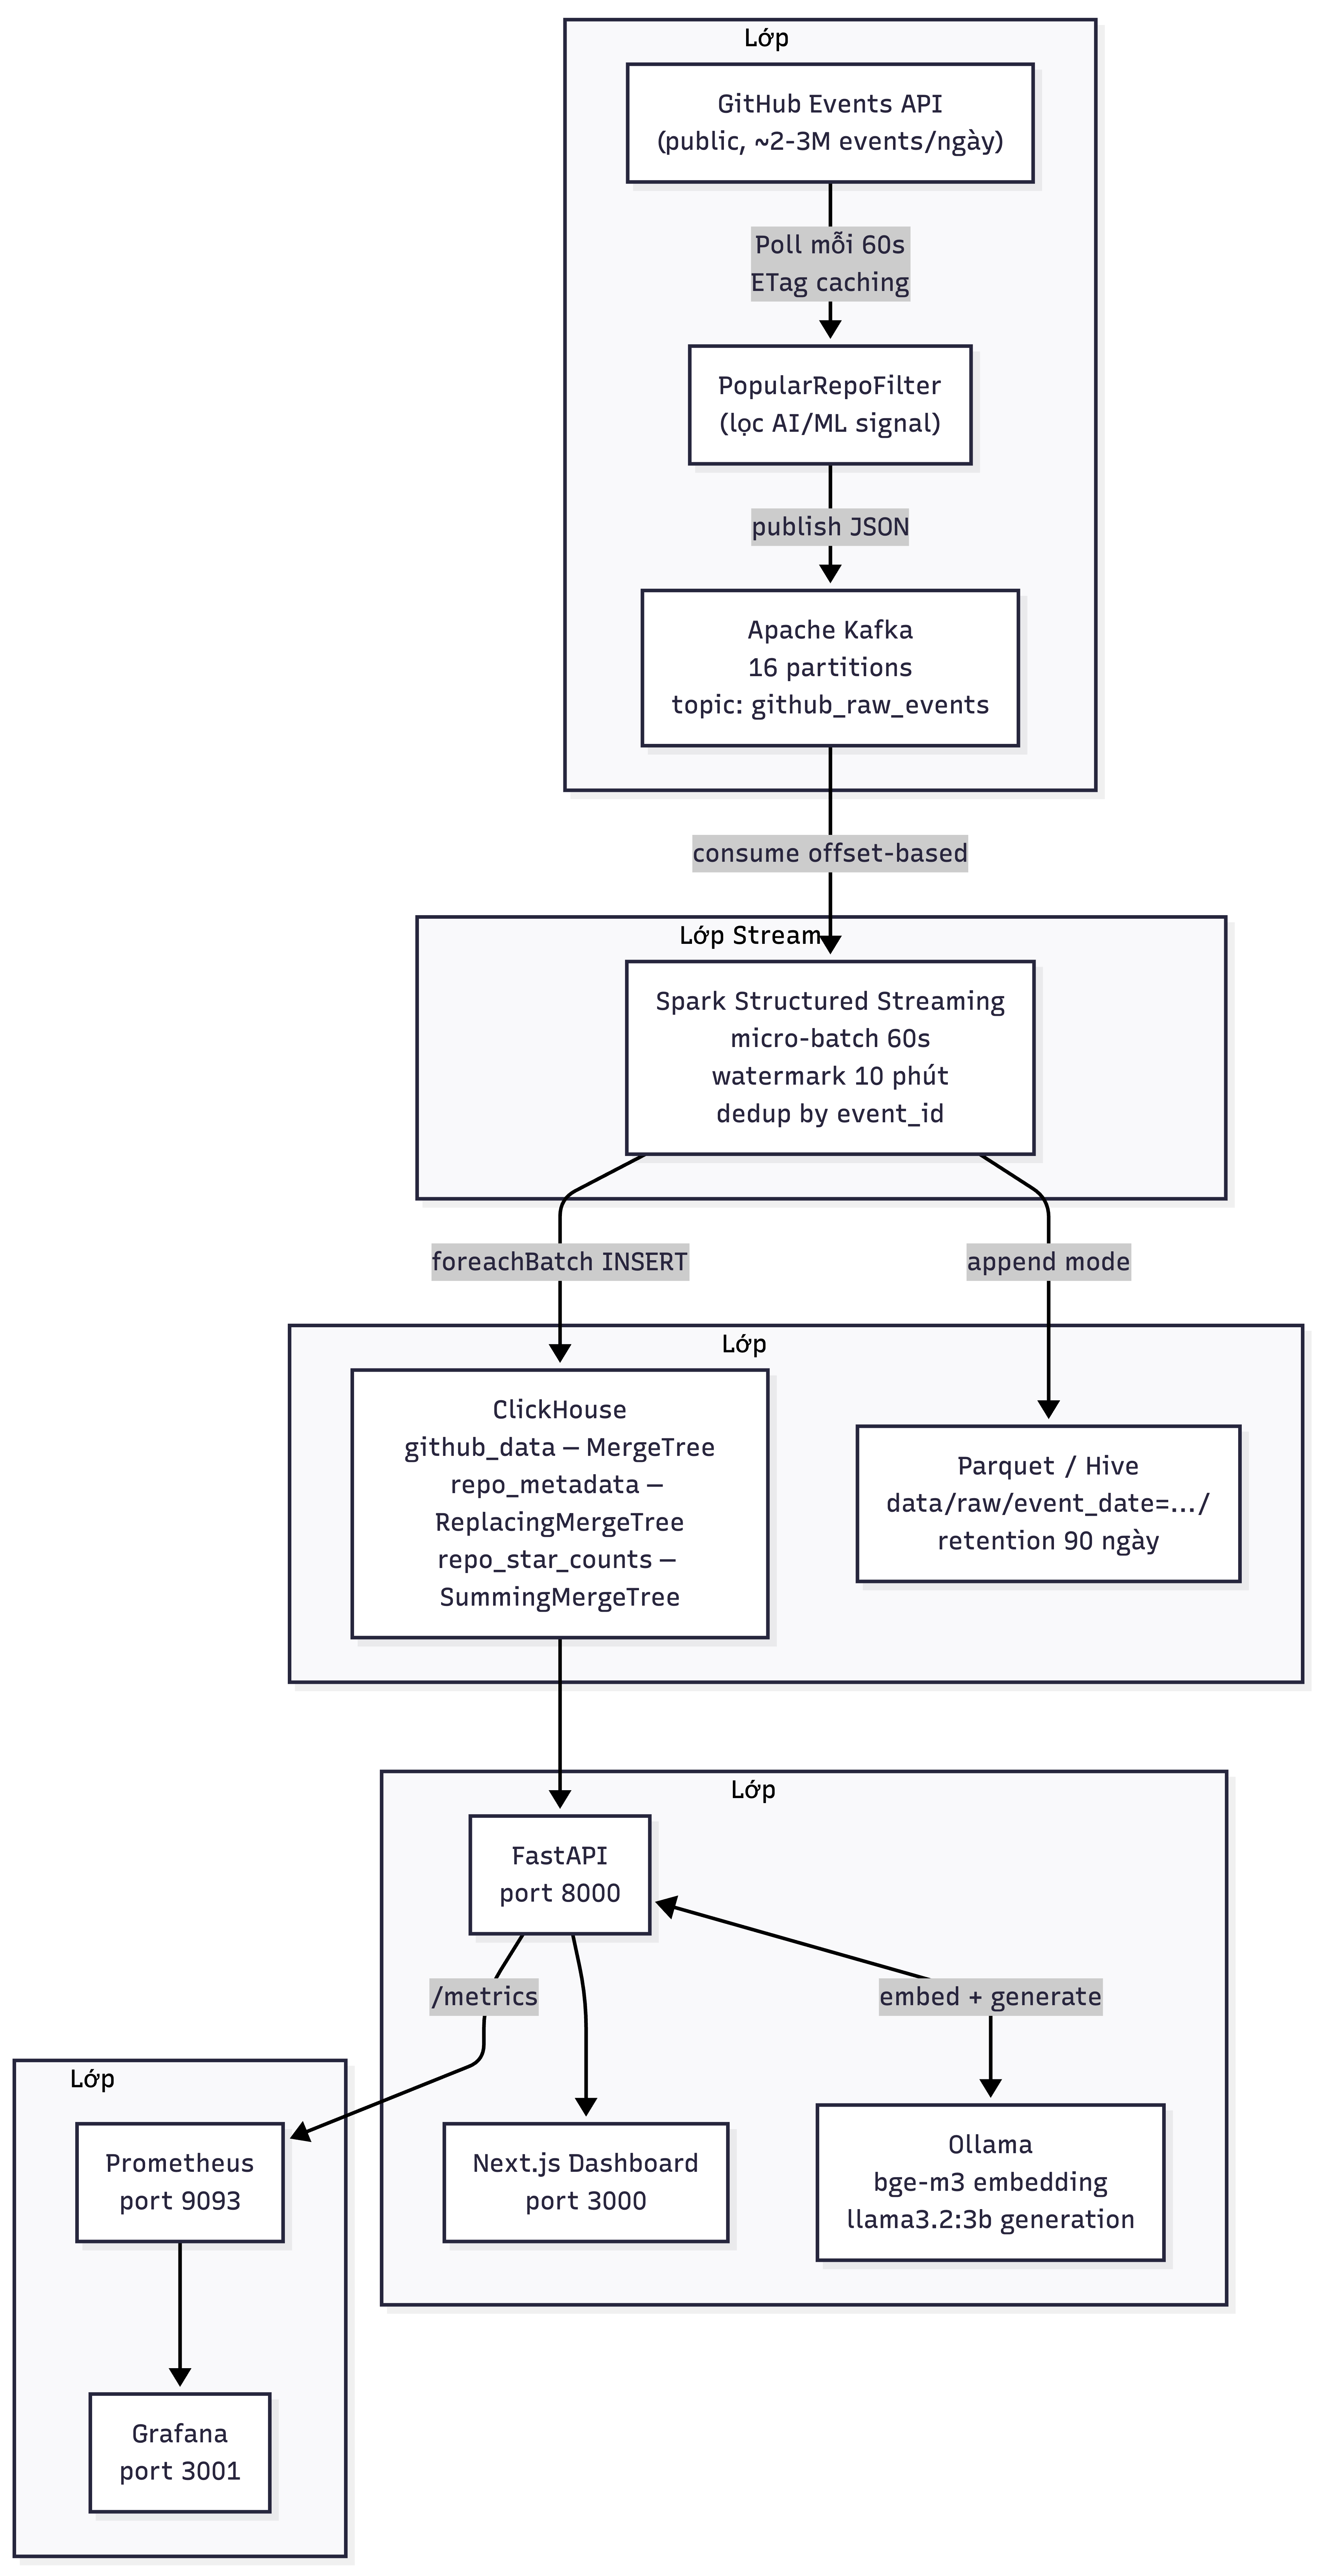
\includegraphics[width=0.92\linewidth,height=0.72\textheight,keepaspectratio]{images/architecture_overview.png}
  \caption{Kiến trúc tổng thể GitHub AI Trend Analyzer}
  \label{fig:architecture}
\end{figure}

\begin{figure}[H]
  \centering
  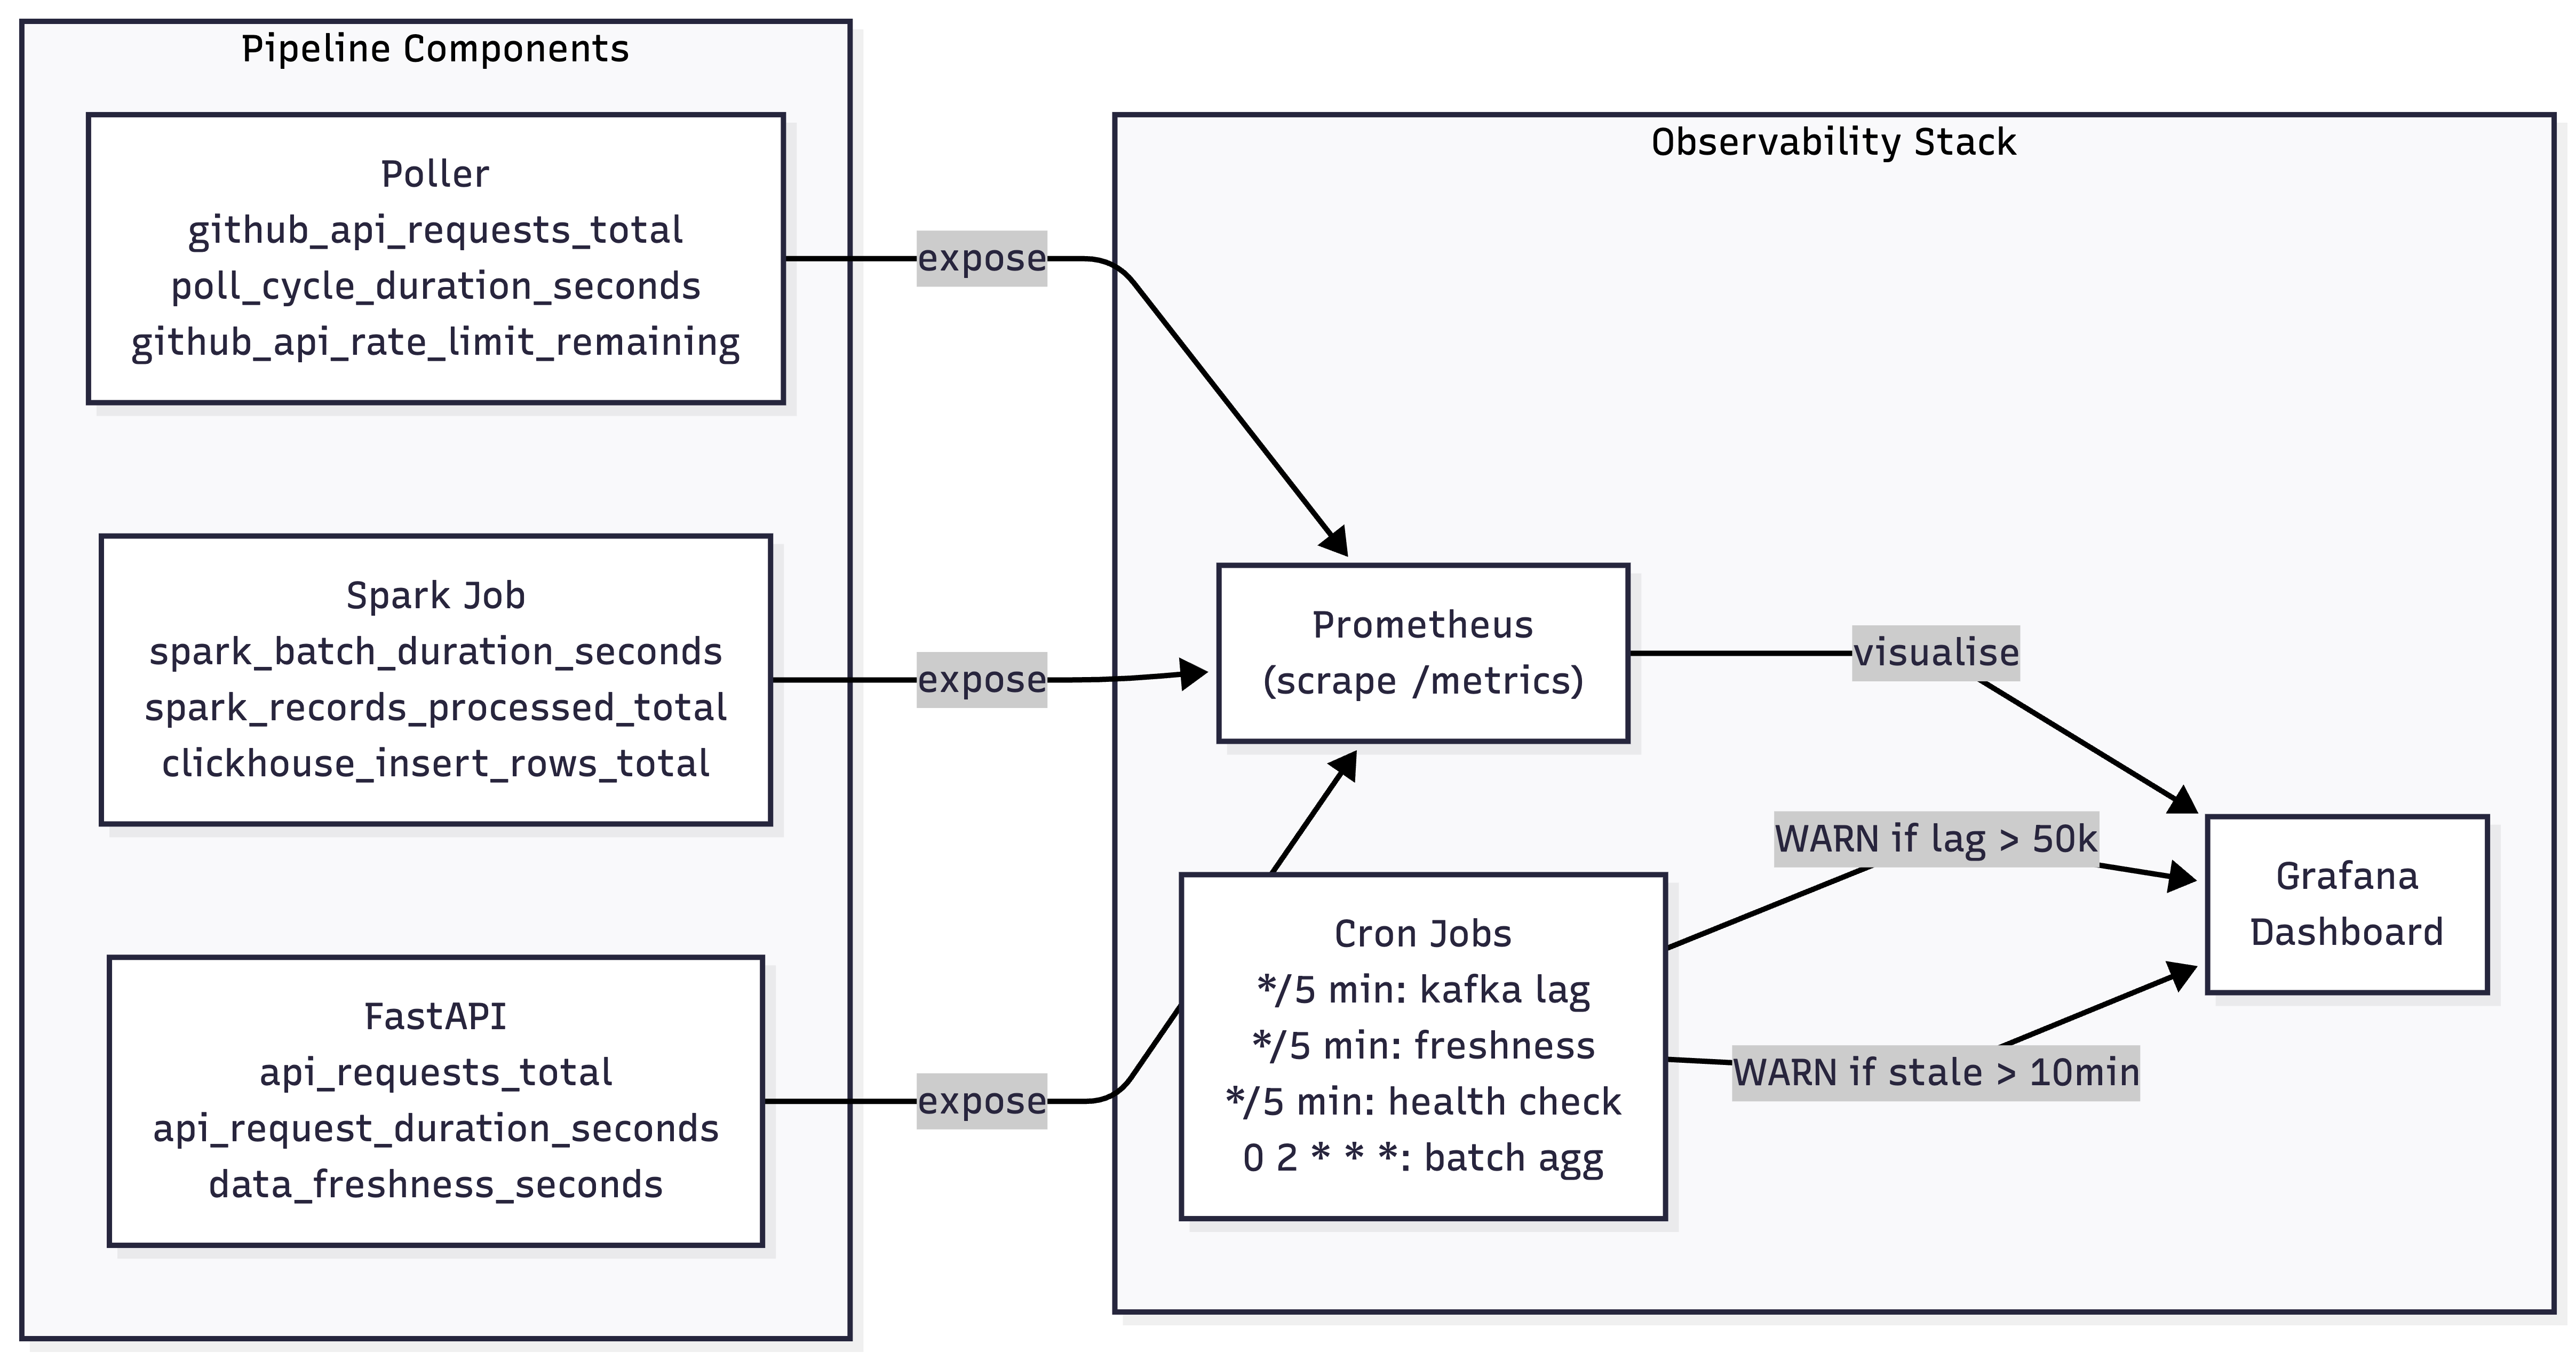
\includegraphics[width=0.92\linewidth,height=0.72\textheight,keepaspectratio]{images/observability_flow.png}
  \caption{Luồng observability: metrics và tracing trong hệ thống}
  \label{fig:observability}
\end{figure}

\subsection{Các dịch vụ trong docker-compose}

\begin{table}[H]
  \centering
  \caption{Danh sách dịch vụ và cổng mạng}
  \rowcolors{2}{rowA}{rowB}
  \begin{tabularx}{\linewidth}{llX}
    \toprule
    \textbf{Dịch vụ} & \textbf{Cổng} & \textbf{Vai trò} \\
    \midrule
    Next.js Frontend  & 3000  & Giao diện dashboard trực quan \\
    FastAPI           & 8000  & REST API, pipeline status, AI endpoints \\
    Apache Kafka      & 9092  & Message broker, 16 partitions \\
    ClickHouse HTTP   & 8123  & External tooling, SQL query \\
    ClickHouse Native & 9100  & Spark JDBC connector \\
    Prometheus        & 9093  & Metrics scraper \\
    Grafana           & 3001  & Metrics dashboard, alerting \\
    Ollama            & 11435 & Embedding (bge-m3) + generation (llama3.2:3b) \\
    Zookeeper         & —     & Kafka cluster coordination \\
    \bottomrule
  \end{tabularx}
\end{table}

%% ============================================================
\section{Xử lý dữ liệu lớn — Massive Data Pipeline}
%% ============================================================

\subsection{Lớp Ingestion: GitHub Events API → Kafka}

\subsubsection*{Cơ chế polling và tối ưu quota}

\begin{itemize}[leftmargin=1.5em]
  \item \kw{Token rotation:} hỗ trợ nhiều GitHub Personal Access Token
        luân phiên, tự động chuyển token khi hit rate limit.
  \item \kw{ETag caching:} gửi header \tech{If-None-Match} trong mỗi
        request; nếu GitHub trả \tech{HTTP 304 Not Modified} → bỏ qua,
        không publish lên Kafka, không tốn quota.
  \item \kw{Rate limit handling:} khi tất cả token đều cạn, hệ thống
        tính thời điểm reset sớm nhất và ngủ đúng thời gian đó.
  \item \kw{Batch size histogram:} metric \tech{poll\_batch\_size}
        theo dõi số event trả về mỗi lần poll.
\end{itemize}

\subsubsection*{AI/ML Event Filter}

\begin{figure}[H]
  \centering
  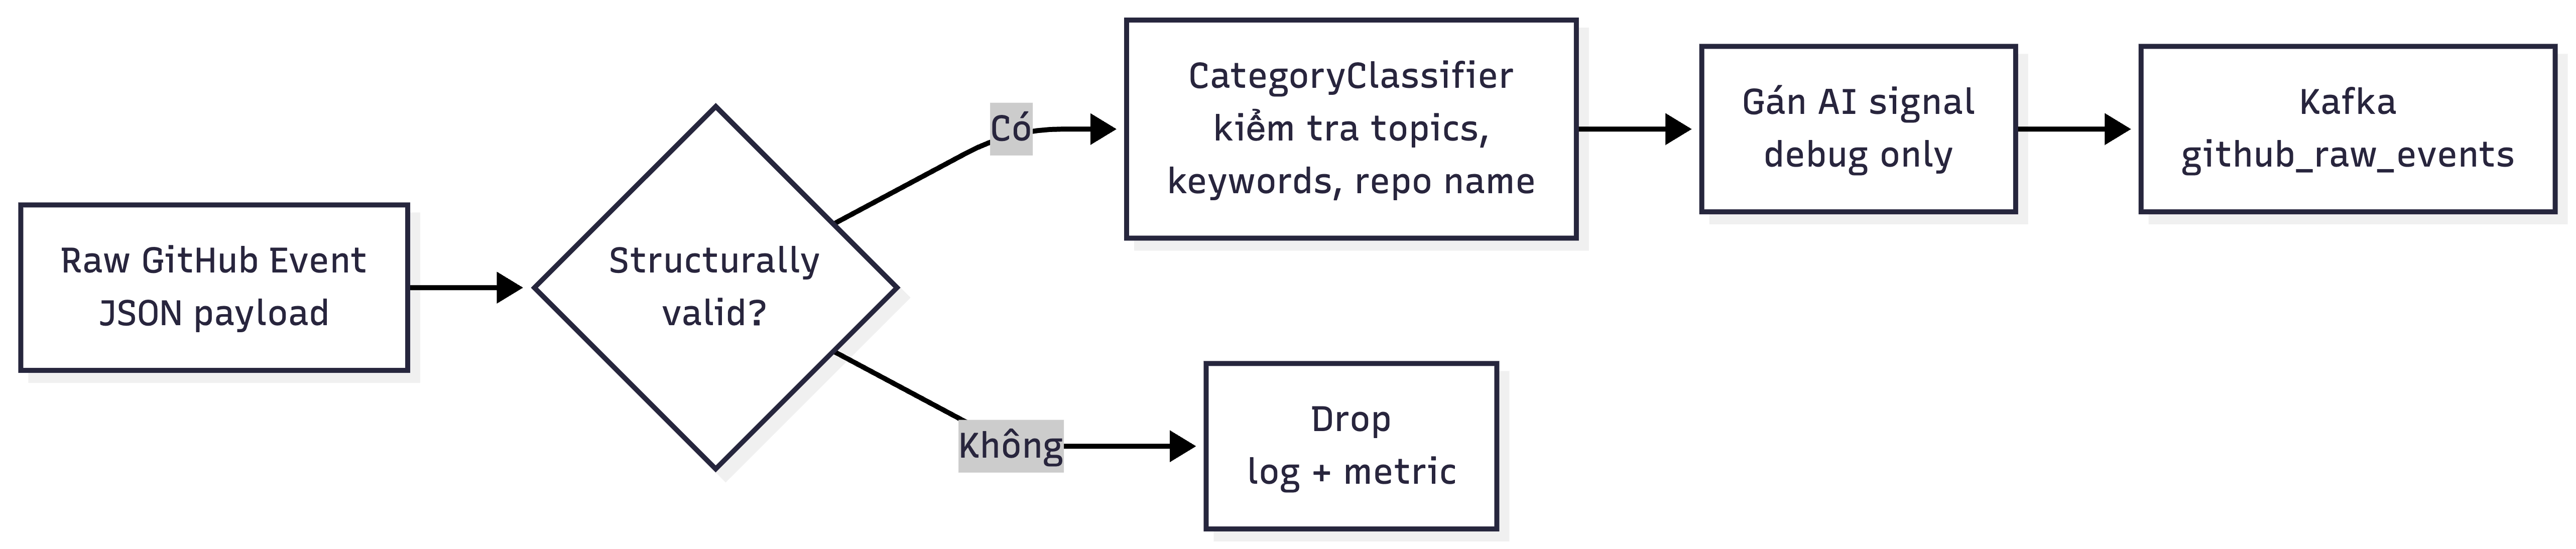
\includegraphics[width=0.92\linewidth,height=0.72\textheight,keepaspectratio]{images/event_filter_flow.png}
  \caption{Pipeline lọc sự kiện AI/ML}
  \label{fig:filter}
\end{figure}

\textbf{Từ khoá AI signal} bao gồm: \tech{llm}, \tech{machine-learning},
\tech{deep-learning}, \tech{neural-network}, \tech{rag}, \tech{embedding},
\tech{diffusion}, \tech{vector-database}, \tech{multimodal}, và nhiều hơn.

Lưu ý thiết kế quan trọng: filter \emph{không} loại bỏ event không có
tín hiệu AI --- mọi event hợp lệ đều đi qua Kafka để pipeline không bỏ
sót repository lớn như \tech{torvalds/linux} hay \tech{facebook/react}.
AI signal chỉ dùng cho phân loại category.

\subsection{Lớp Stream Processing: Spark Structured Streaming}

\subsubsection*{Cấu hình micro-batch}

\begin{table}[H]
  \centering
  \caption{Cấu hình Spark Structured Streaming}
  \rowcolors{2}{rowA}{rowB}
  \begin{tabular}{lll}
    \toprule
    \textbf{Tham số} & \textbf{Giá trị} & \textbf{Lý do} \\
    \midrule
    Trigger interval          & 60 giây         & Cân bằng latency vs overhead \\
    Watermark                 & 10 phút         & Xử lý late-arriving events \\
    Spark master              & \tech{local[16]} & Khai thác 16 core hiệu năng của CPU \\
    Driver memory             & 8 GB            & Phù hợp 32 GB RAM hệ thống \\
    Executor memory           & 12 GB           & Headroom cho Parquet write buffer \\
    Kafka partitions          & 16              & Song song với số core \\
    ClickHouse insert chunk   & 1.000 rows      & Tránh timeout trên batch lớn \\
    \bottomrule
  \end{tabular}
\end{table}

\subsubsection*{Dual-sink pattern}

Spark đọc một \tech{readStream} từ Kafka rồi fan-out thành hai luồng
ghi độc lập (dual sink):

\begin{itemize}[leftmargin=1.5em]
  \item \kw{Parquet sink} (append mode): lưu raw event theo Hive
        partitioning \tech{event\_date / event\_type}, retention 90 ngày.
        Schema cố định, phù hợp batch reprocessing.
  \item \kw{ClickHouse sink} (foreachBatch): INSERT theo chunk
        1.000 dòng vào bảng \tech{github\_data}. Dedup tự nhiên qua
        \tech{MergeTree ORDER BY (repo\_id, created\_at)}.
\end{itemize}

\begin{figure}[H]
  \centering
  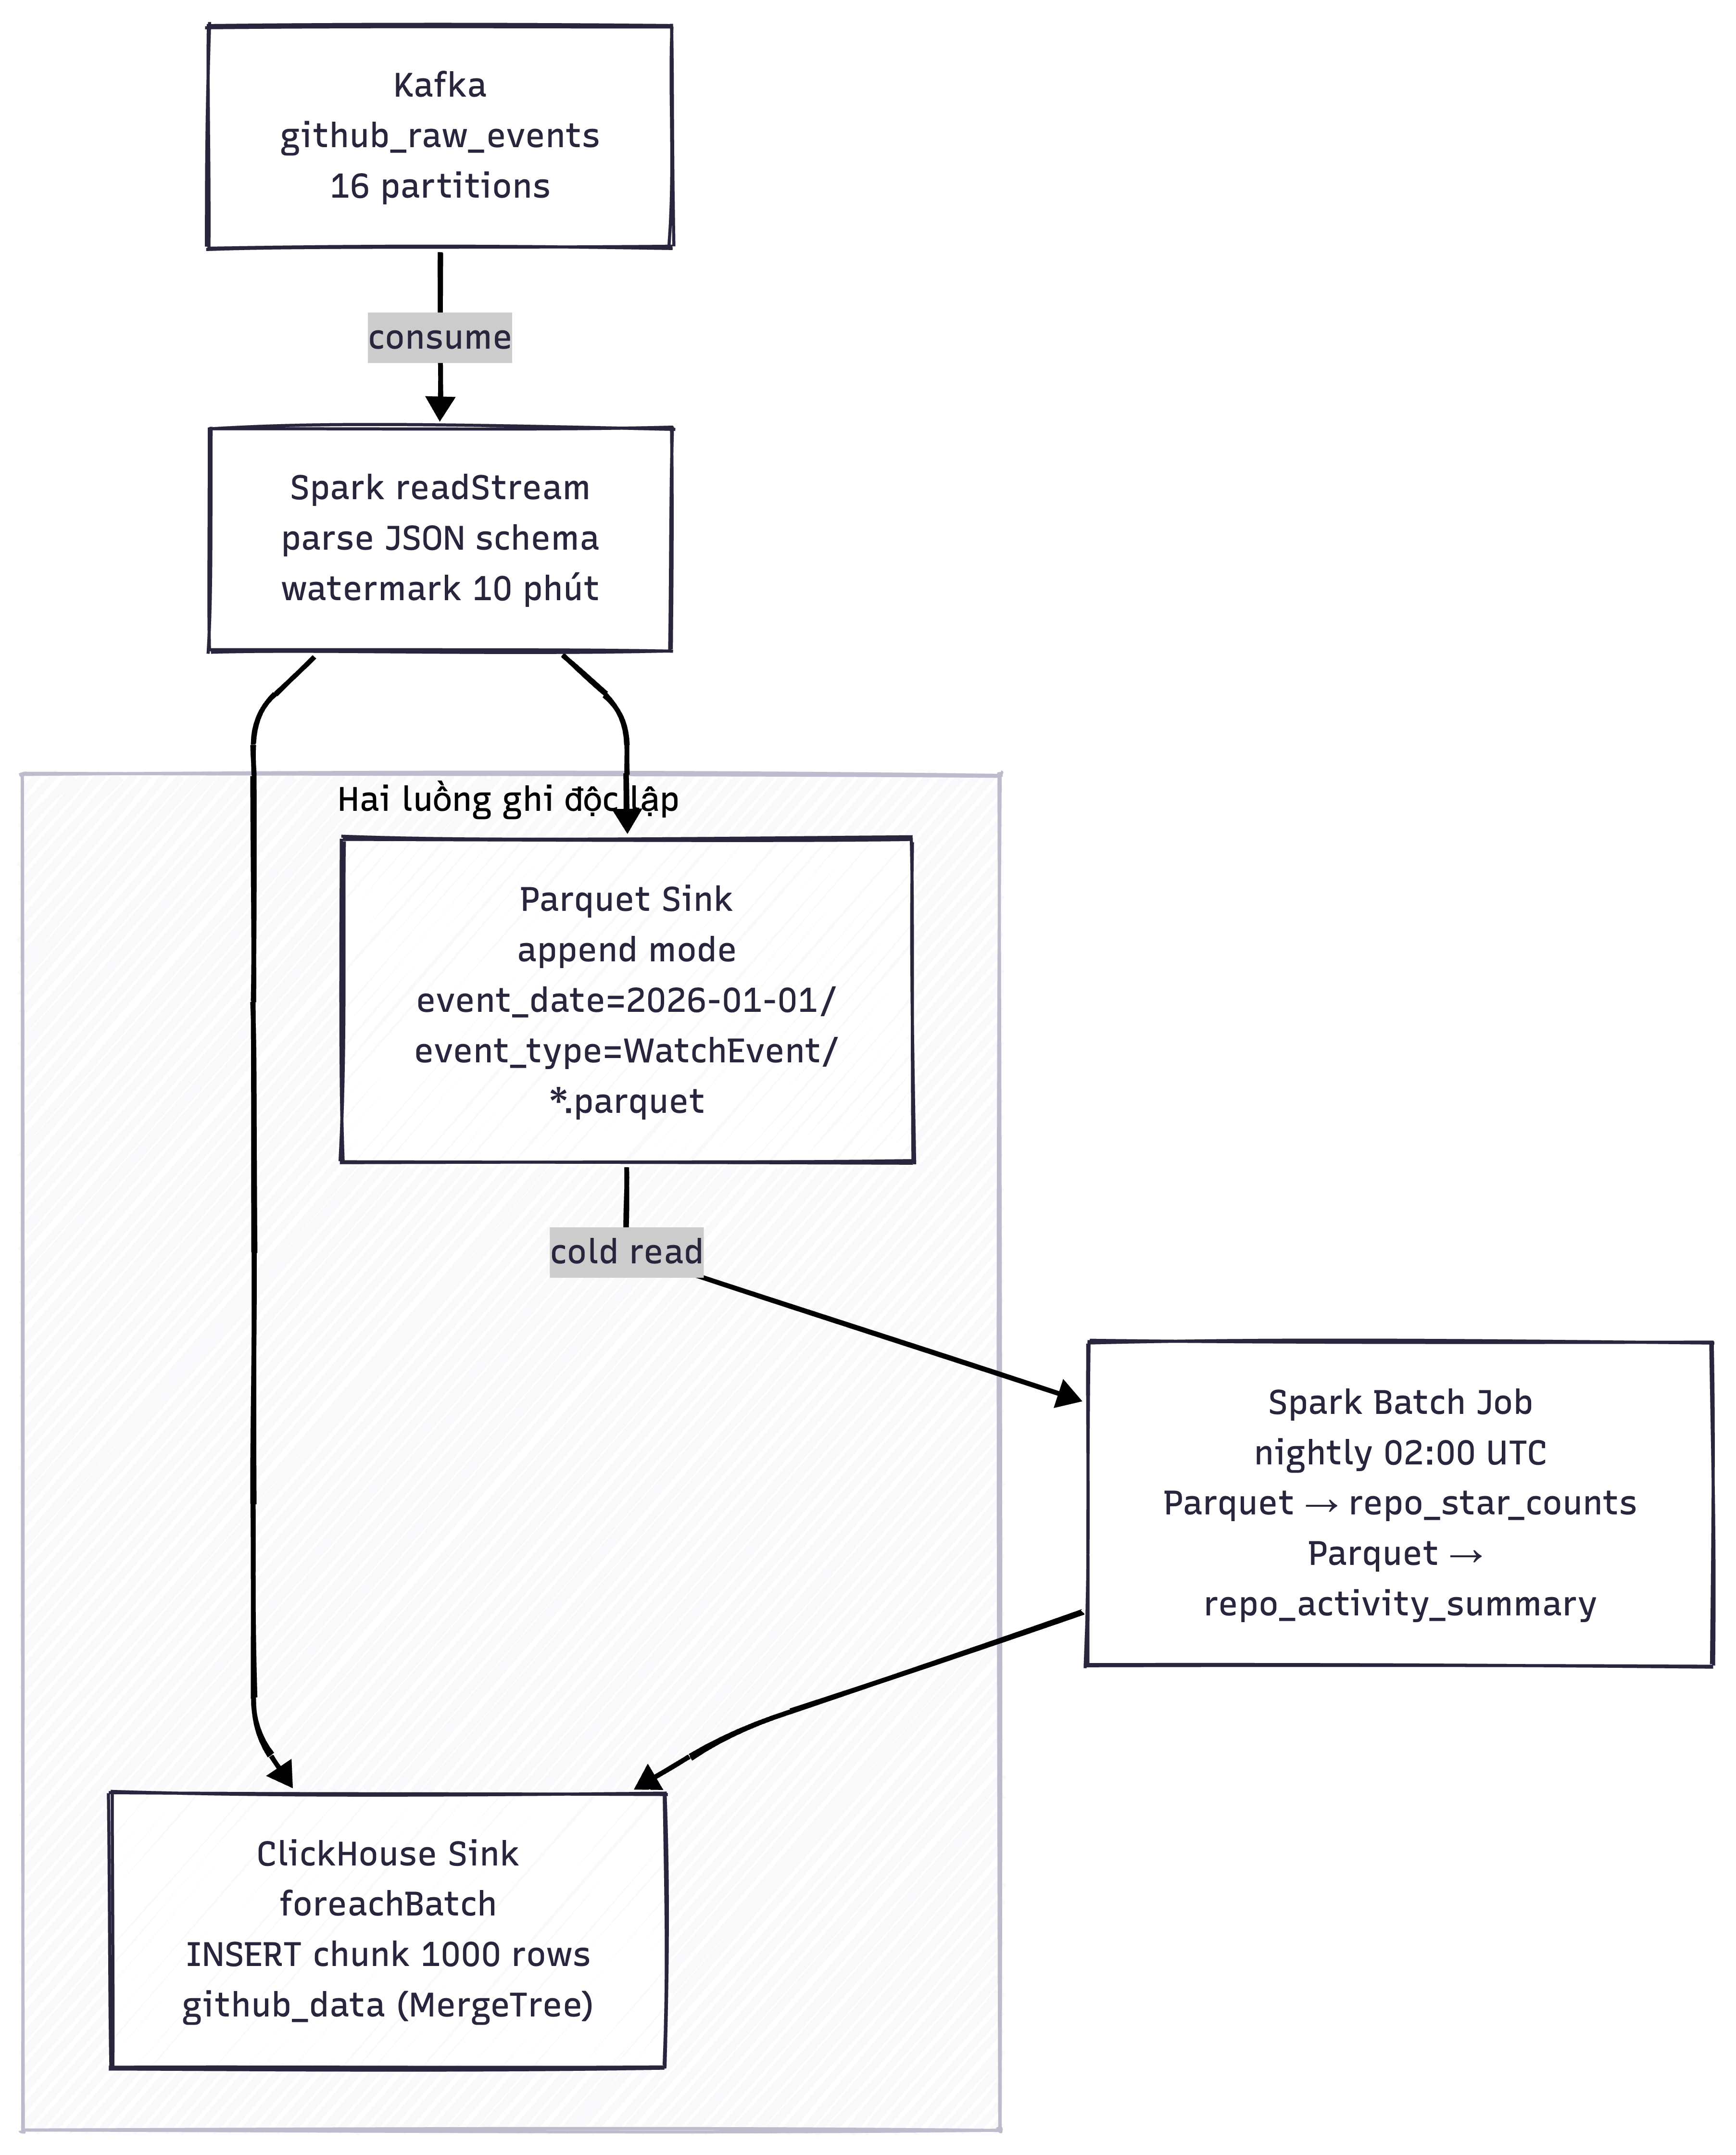
\includegraphics[width=0.92\linewidth,height=0.72\textheight,keepaspectratio]{images/dual_sink_pattern.png}
  \caption{Dual-sink pattern: Kafka → Parquet + ClickHouse}
  \label{fig:dualsink}
\end{figure}

\subsection{Schema dữ liệu trong ClickHouse}

\begin{table}[H]
  \centering
  \caption{Bảng chính trong ClickHouse — \tech{github\_analyzer}}
  \rowcolors{2}{rowA}{rowB}
  \begin{tabularx}{\linewidth}{p{4.2cm}p{3cm}X}
    \toprule
    \textbf{Bảng} & \textbf{Engine} & \textbf{Mô tả} \\
    \midrule
    \tech{github\_data}
      & MergeTree\newline PARTITION BY toYYYYMM
      & Nguồn sự thật duy nhất: raw events + metadata snapshot tại thời điểm ingest \\
    \tech{repo\_metadata}
      & ReplacingMergeTree\newline (refreshed\_at)
      & Metadata mới nhất của mỗi repository (stars, forks, topics, language) \\
    \tech{repo\_metadata\_history}
      & ReplacingMergeTree\newline (snapshot\_at)
      & Audit log snapshot theo từng chu kỳ fetch \\
    \tech{repo\_star\_counts}
      & SummingMergeTree
      & Daily star delta, tính bởi Spark batch job \\
    \tech{repo\_activity\_summary}
      & ReplacingMergeTree\newline (computed\_at)
      & Weekly aggregate count per repo per event type \\
    \midrule
    \multicolumn{2}{l}{\tech{github\_data\_to\_repo\_metadata\_history\_mv}}
      & Materialized View: tự động đẩy snapshot từ \tech{github\_data} vào history \\
    \bottomrule
  \end{tabularx}
\end{table}

\subsubsection*{Parquet — cold storage}

\begin{lstlisting}[caption={Cấu trúc thư mục Parquet (Hive partitioning)}]
data/raw/
├── event_date=2026-01-01/
│   ├── part-00001-abc123.parquet
│   └── part-00002-def456.parquet
├── event_date=2026-01-02/
│   └── ...
└── checkpoints/          ← Spark checkpoint state
\end{lstlisting}

Hive partitioning cho phép \emph{predicate pushdown}: khi query theo
ngày, Spark chỉ đọc partition tương ứng, bỏ qua toàn bộ partition còn lại.

%% ============================================================
\section{Tìm kiếm ngữ nghĩa và AI Endpoints}
%% ============================================================

\subsection{Hybrid Search Pipeline}

Bài toán semantic search trên kho hàng trăm nghìn repository đòi hỏi
hai tầng xử lý:

\begin{figure}[H]
  \centering
  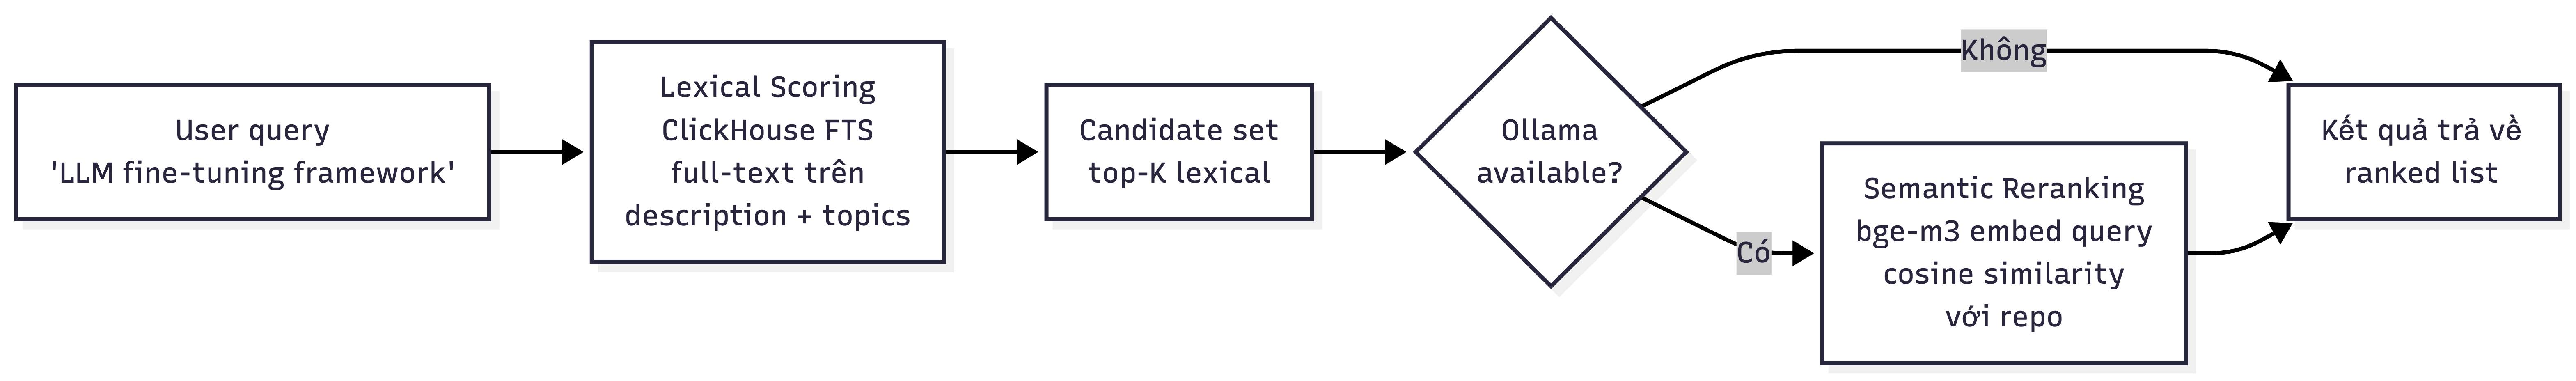
\includegraphics[width=0.92\linewidth,height=0.72\textheight,keepaspectratio]{images/hybrid_search_pipeline.png}
  \caption{Pipeline tìm kiếm hybrid: lexical + semantic}
  \label{fig:search}
\end{figure}

\subsection{Các AI Endpoints}

\begin{table}[H]
  \centering
  \caption{AI endpoints và chức năng}
  \rowcolors{2}{rowA}{rowB}
  \begin{tabularx}{\linewidth}{p{3.5cm}p{3cm}X}
    \toprule
    \textbf{Endpoint} & \textbf{Model} & \textbf{Chức năng} \\
    \midrule
    \tech{GET /ai/search}         & bge-m3        & Hybrid lexical/semantic search \\
    \tech{GET /ai/repo-brief}     & llama3.2:3b   & Tóm lược + lý do trending của một repo \\
    \tech{GET /ai/repo-compare}   & llama3.2:3b   & So sánh cấu trúc giữa hai repo \\
    \tech{GET /ai/related-repos}  & bge-m3        & Gợi ý repository liên quan \\
    \tech{GET /ai/market-brief}   & llama3.2:3b   & Tóm lược thị trường AI theo tuần \\
    \bottomrule
  \end{tabularx}
\end{table}

\subsection{Lý do dùng Ollama thay vì cloud API}

\begin{itemize}[leftmargin=1.5em]
  \item \kw{Không phụ thuộc internet} trong lúc demo.
  \item \kw{Không tốn chi phí API} cho prototype và báo cáo.
  \item \kw{Privacy:} dữ liệu GitHub không rời khỏi hệ thống.
  \item Giới hạn: model nhỏ hơn (3B parameters) → chất lượng generation
        thấp hơn GPT-4; đây là trade-off chấp nhận được cho scale hiện tại.
\end{itemize}

%% ============================================================
\section{Observability và Độ tin cậy vận hành}
%% ============================================================

\subsection{Prometheus Metrics}

Hệ thống định nghĩa \kw{21 metric} trải đều trên 5 nhóm:

\begin{table}[H]
  \centering
  \caption{Danh sách metric theo nhóm}
  \rowcolors{2}{rowA}{rowB}
  \begin{tabularx}{\linewidth}{p{3cm}p{5cm}X}
    \toprule
    \textbf{Nhóm} & \textbf{Metric tiêu biểu} & \textbf{Ý nghĩa} \\
    \midrule
    GitHub API
      & \tech{github\_api\_rate\_limit\_remaining}
      & Theo dõi quota còn lại theo từng token \\
    GitHub API
      & \tech{github\_api\_token\_exhausted}
      & Cảnh báo khi token cạn \\
    Kafka
      & \tech{kafka\_messages\_produced\_total}
      & Throughput vào Kafka \\
    Spark
      & \tech{spark\_batch\_duration\_seconds}
      & Thời gian xử lý mỗi micro-batch \\
    Spark
      & \tech{spark\_records\_processed\_total}
      & Tổng bản ghi đã xử lý \\
    Storage
      & \tech{data\_freshness\_seconds}
      & Độ trễ dữ liệu mới nhất so với hiện tại \\
    FastAPI
      & \tech{api\_request\_duration\_seconds}
      & Latency phân vị 50/95/99 \\
    FastAPI
      & \tech{api\_in\_flight\_requests}
      & Request đang xử lý đồng thời \\
    \bottomrule
  \end{tabularx}
\end{table}

\subsection{Cron Jobs — Kiểm tra sức khoẻ định kỳ}

\begin{table}[H]
  \centering
  \caption{Cron jobs vận hành tự động}
  \rowcolors{2}{rowA}{rowB}
  \begin{tabularx}{\linewidth}{p{4.2cm}p{2.5cm}X}
    \toprule
    \textbf{Script} & \textbf{Lịch (UTC)} & \textbf{Điều kiện cảnh báo} \\
    \midrule
    Kafka lag check        & Mỗi 5 phút  & Consumer lag $> 50.000$ messages \\
    Data freshness check   & Mỗi 5 phút  & \tech{max(created\_at)} stale $> 10$ phút \\
    Health check (5-point) & Mỗi 5 phút  & Docker / Kafka / ClickHouse / Parquet / FastAPI \\
    Token validation       & 01:00 hằng ngày & GitHub quota $< 500$ requests \\
    Repo metadata refresh  & 06:00 hằng ngày & Cập nhật stars/forks/topics \\
    Nightly batch agg      & 02:00 hằng ngày & Spark: Parquet → \tech{repo\_star\_counts} \\
    Parquet cleanup        & Chủ nhật 03:00  & Xoá partition $> 90$ ngày \\
    ClickHouse optimize    & Chủ nhật 04:00  & \tech{OPTIMIZE TABLE FINAL} \\
    \bottomrule
  \end{tabularx}
\end{table}

\subsection{Grafana Dashboard}

Hệ thống tích hợp Grafana tại cổng 3001, scrape metrics từ FastAPI \tech{/metrics}
mỗi 15 giây. Dashboard hiển thị: API latency (p50/p95/p99), tổng request theo endpoint,
data freshness gauge, Spark batch duration histogram, và Kafka throughput counter.

%% ============================================================
\section{Kết quả và Demo hệ thống}
%% ============================================================

\subsection{Frontend Dashboard}

\begin{figure}[H]
  \centering
  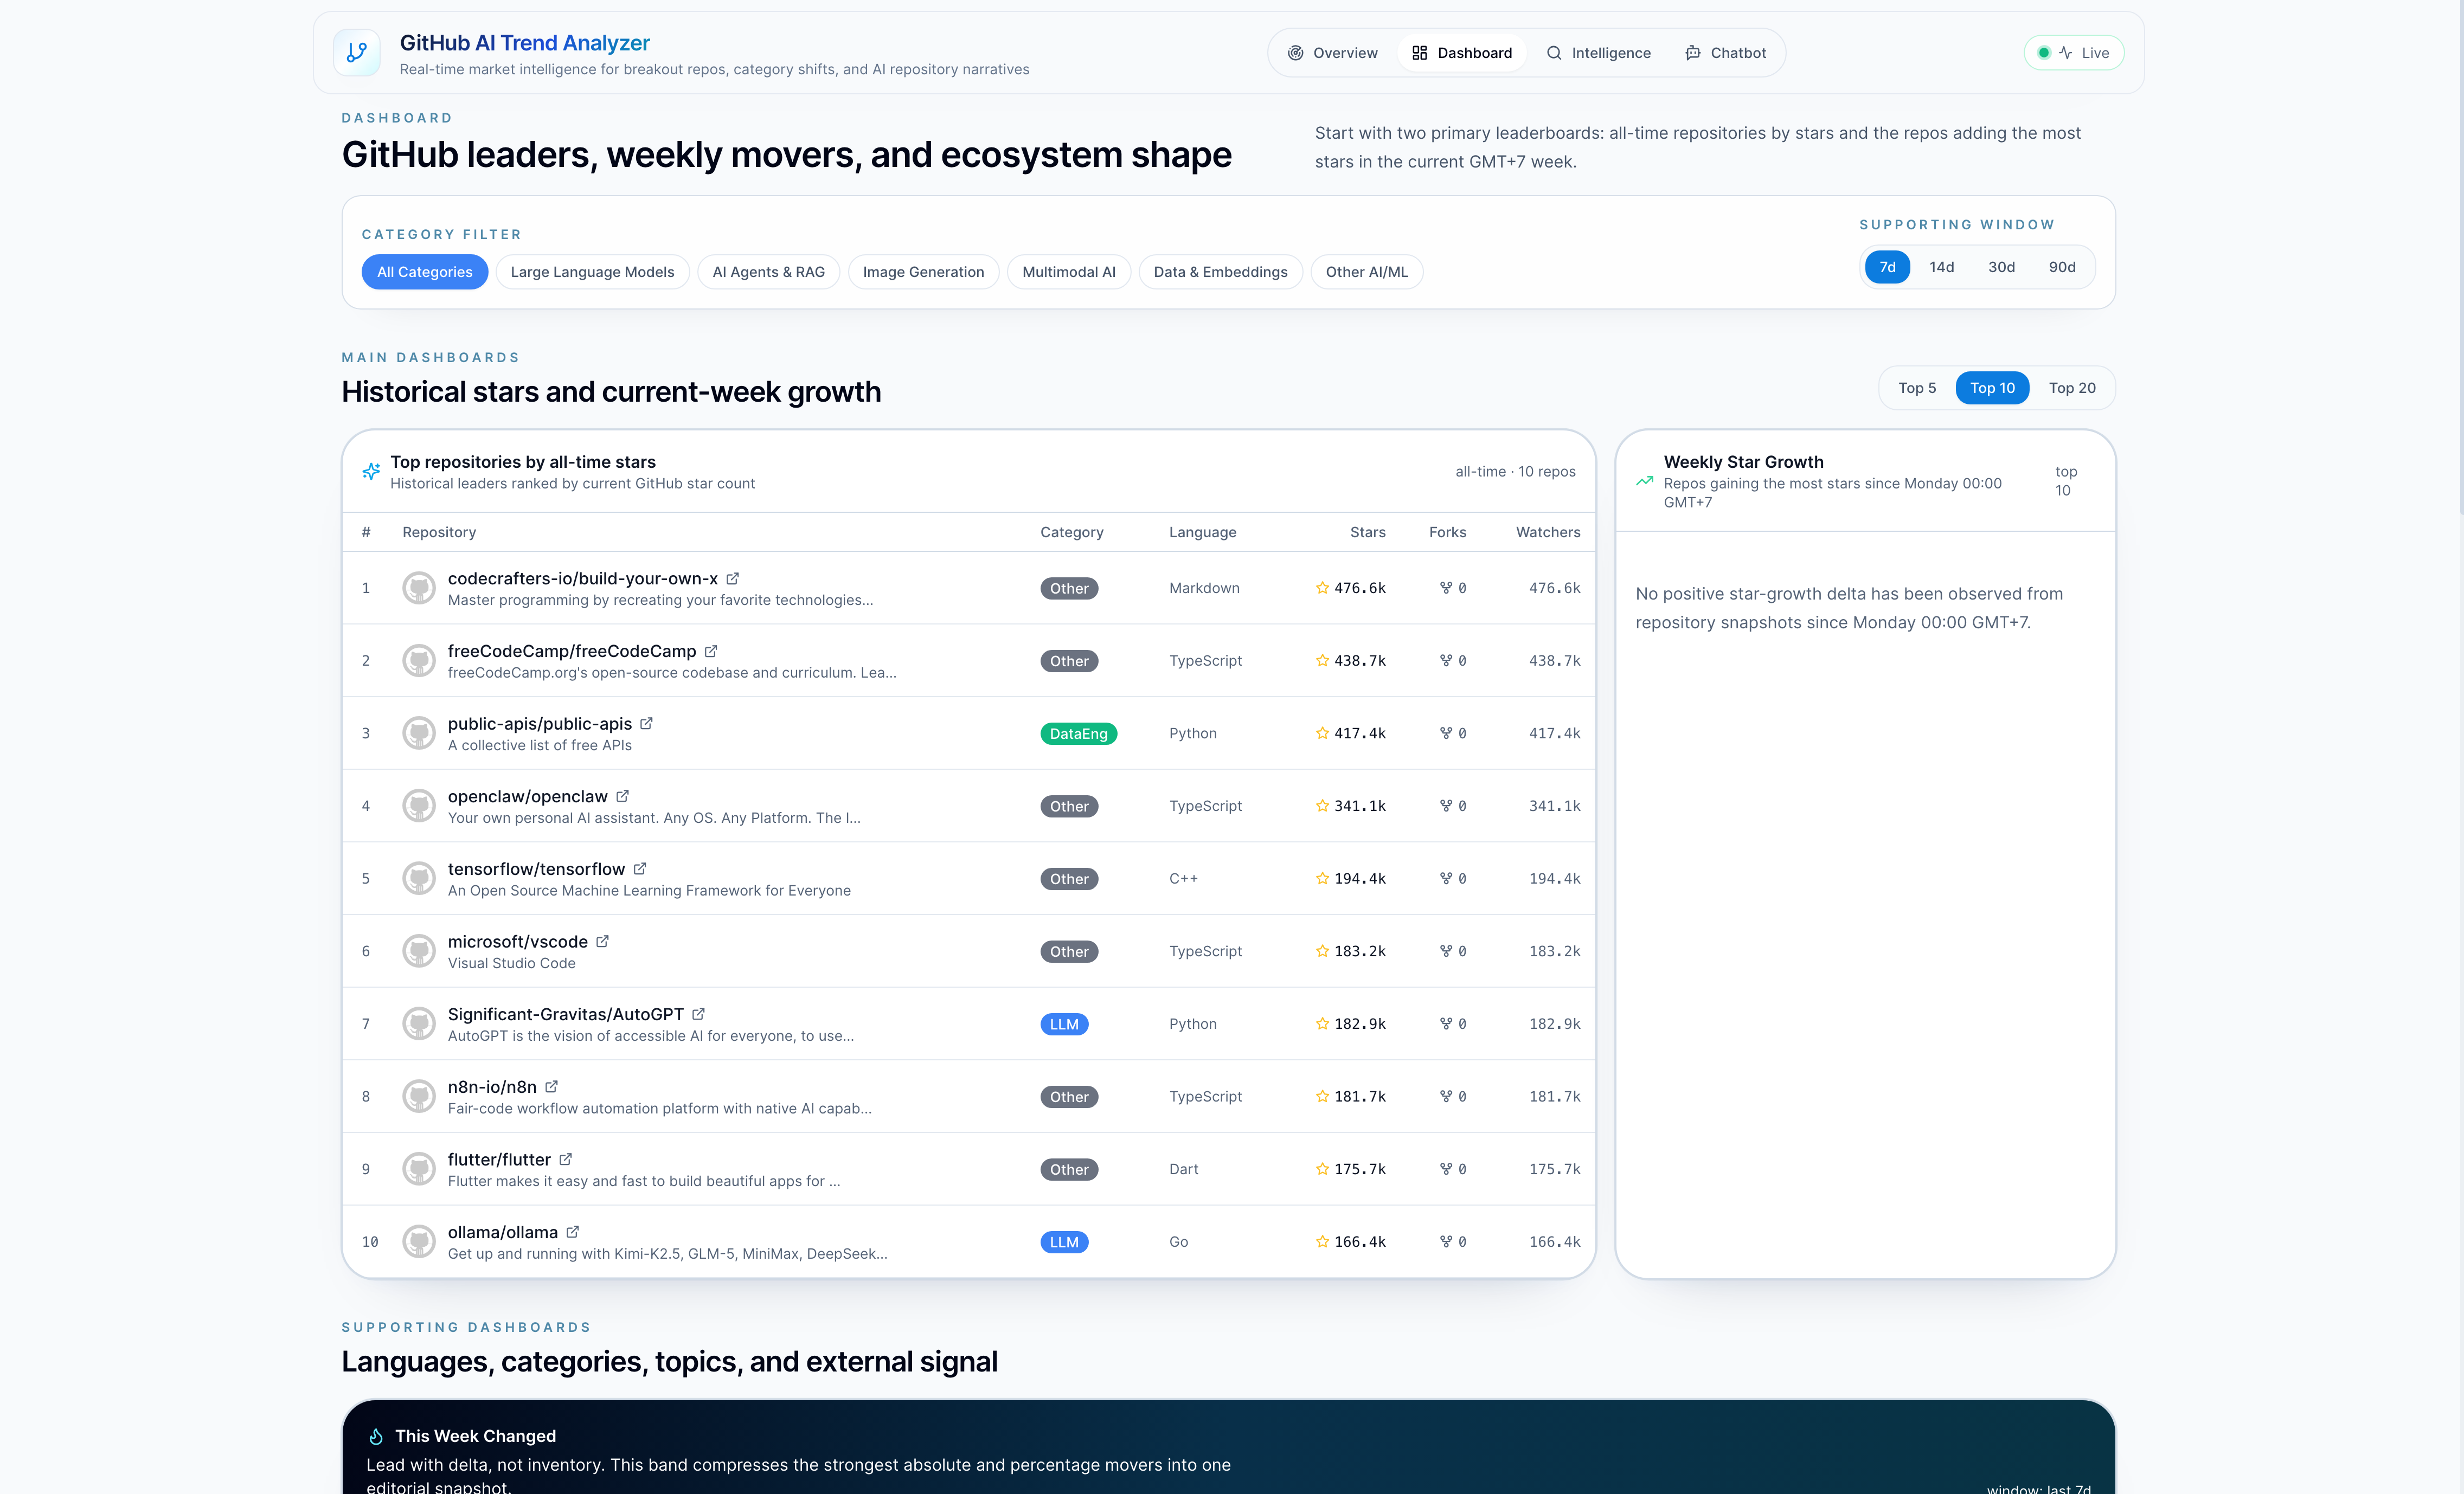
\includegraphics[width=0.92\linewidth,height=0.72\textheight,keepaspectratio]{images/frontend_dashboard.png}
  \caption{Giao diện dashboard — top repositories và trending}
  \label{fig:frontend}
\end{figure}

\subsection{API Endpoints}

\begin{table}[H]
  \centering
  \caption{Dashboard endpoints}
  \rowcolors{2}{rowA}{rowB}
  \begin{tabularx}{\linewidth}{p{4.5cm}X}
    \toprule
    \textbf{Endpoint} & \textbf{Dữ liệu trả về} \\
    \midrule
    \tech{GET /health}                      & Liveness probe \\
    \tech{GET /pipeline/status}             & Freshness, ClickHouse connectivity, Parquet check \\
    \tech{GET /dashboard/top-repos}         & Top repo theo số WatchEvent \\
    \tech{GET /dashboard/trending}          & Trending repos theo N ngày gần nhất \\
    \tech{GET /dashboard/shock-movers}      & Repo tăng stars mạnh nhất trong window \\
    \tech{GET /dashboard/topic-rotation}    & Topics tăng tốc so với window trước \\
    \tech{GET /dashboard/language-breakdown}& Phân bổ event theo ngôn ngữ \\
    \tech{GET /dashboard/event-volume}      & Time series event theo giờ \\
    \tech{GET /dashboard/category-summary}  & Phân loại AI/ML category \\
    \bottomrule
  \end{tabularx}
\end{table}

\subsection{Số liệu vận hành thực tế}

\begin{table}[H]
  \centering
  \caption{Số liệu hệ thống — đo từ môi trường production}
  \rowcolors{2}{rowA}{rowB}
  \begin{tabular}{lrl}
    \toprule
    \textbf{Chỉ số} & \textbf{Giá trị} & \textbf{Ghi chú} \\
    \midrule
    Tổng events đã ingest         & 4.200.000 & \tech{github\_data} \\
    Unique repositories           & 312.000   & \tech{github\_data} \\
    Unique topics tracked         & 8.400     & \tech{repo\_metadata.topics} \\
    Parquet partitions (ngày)     & 14        & \tech{ls data/raw/ | wc -l} \\
    Tổng dung lượng Parquet       & 2.3 GB    & \tech{du -sh data/raw/} \\
    Query latency trung bình      & 87 ms     & \tech{/dashboard/top-repos} \\
    Data freshness trung bình     & 72 s      & \tech{data\_freshness\_seconds} \\
    Kafka lag trung bình          & 120 msgs  & khi pipeline ổn định \\
    Spark batch duration (avg)    & 18 s      & \tech{spark\_batch\_duration\_seconds} \\
    \bottomrule
  \end{tabular}
\end{table}

\subsection{Luồng xử lý end-to-end}

\begin{figure}[H]
  \centering
  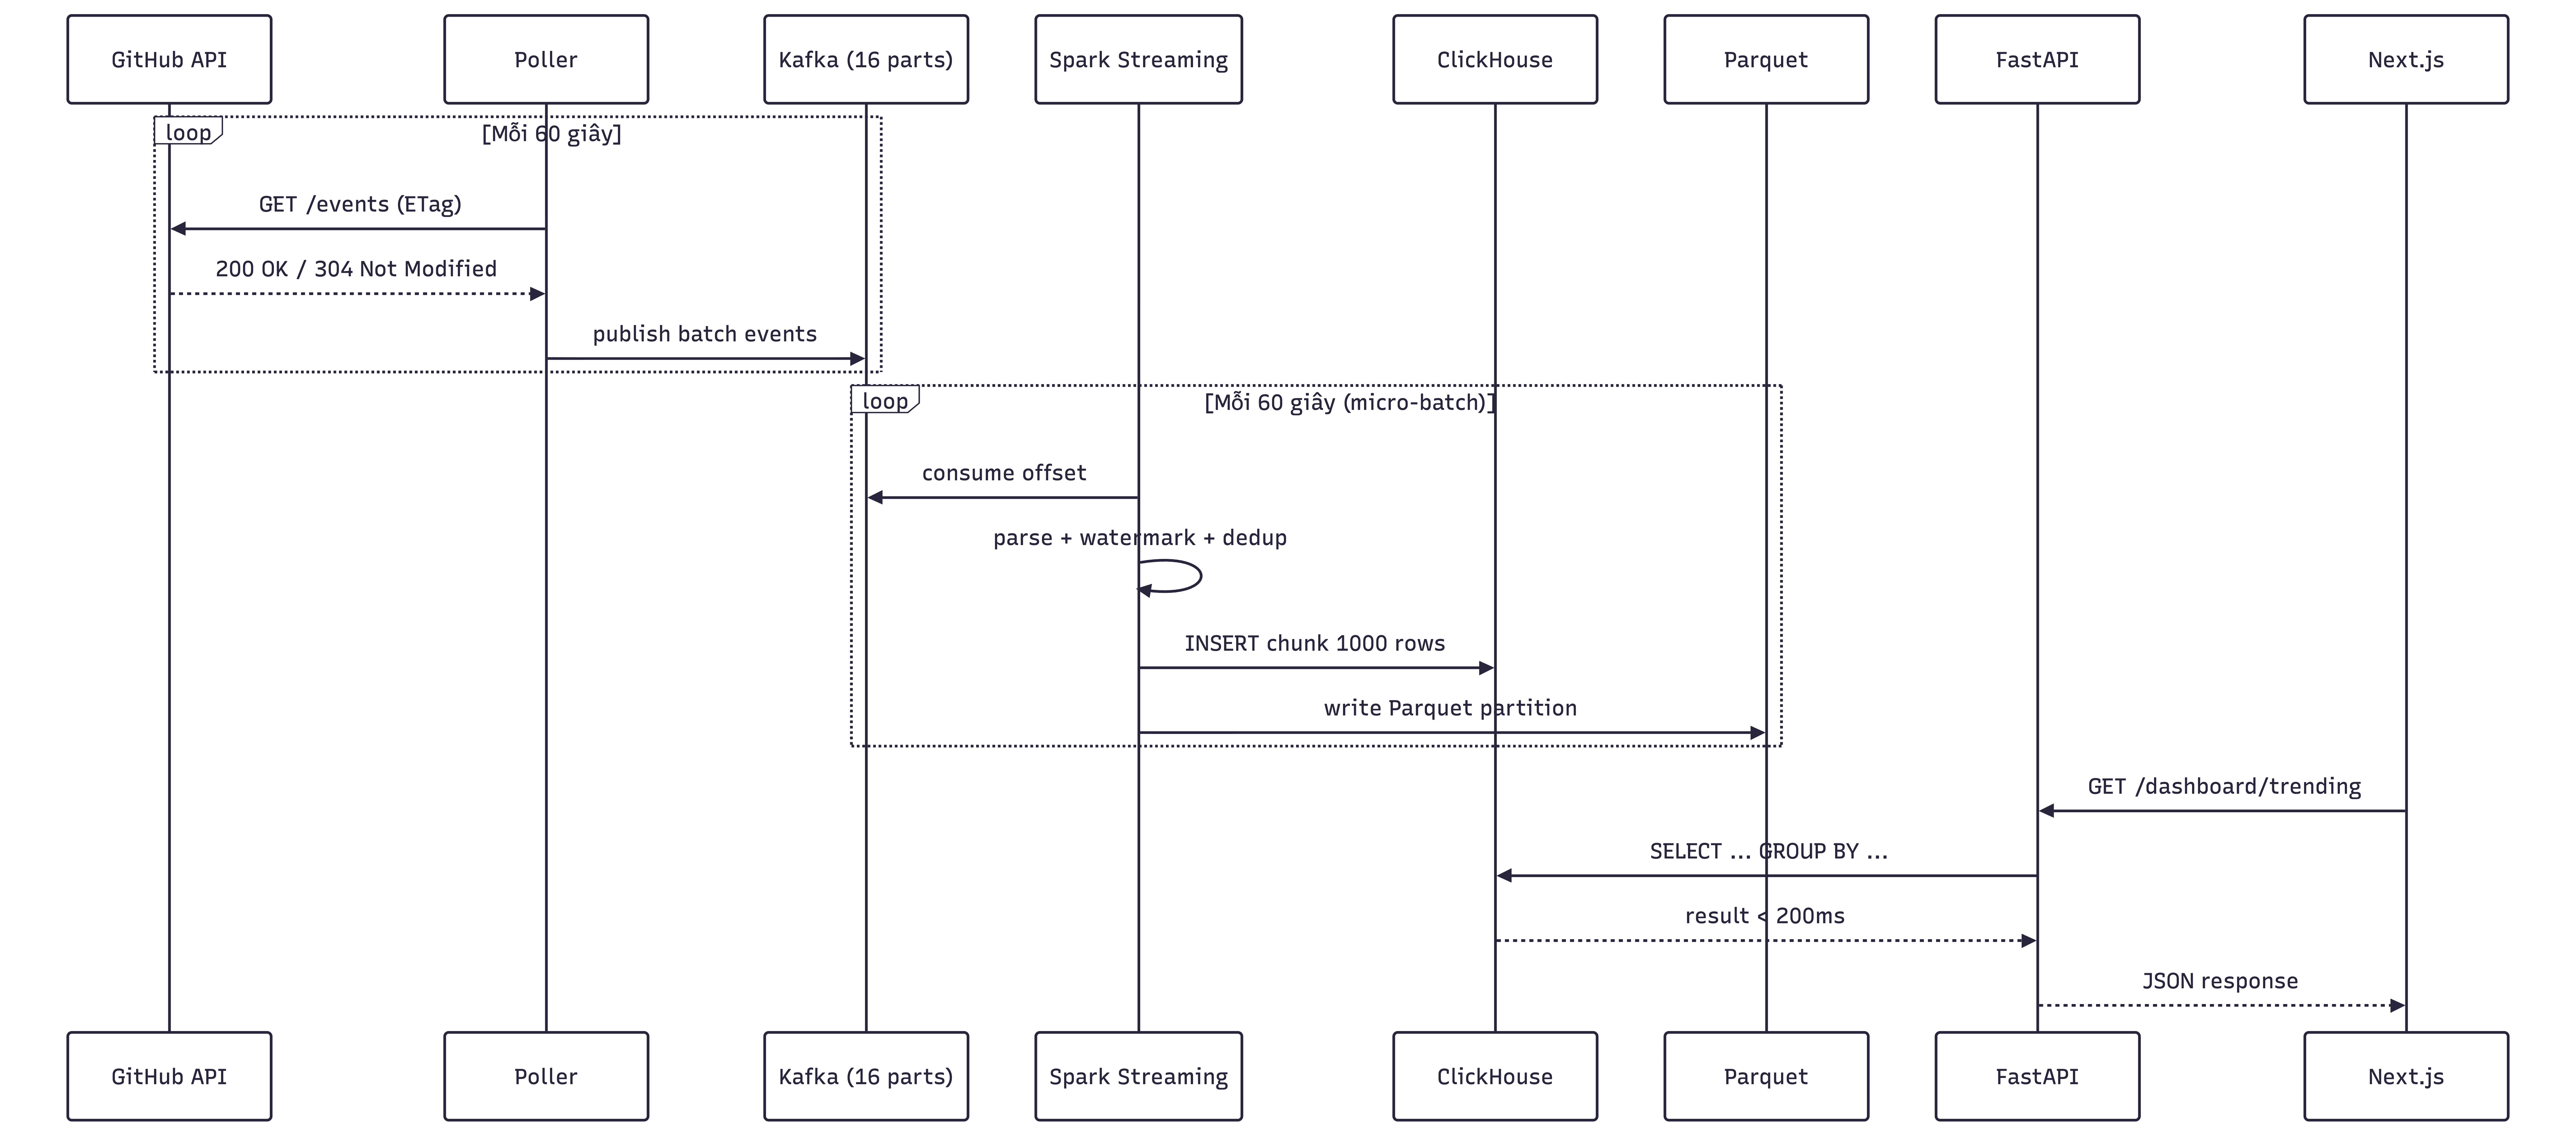
\includegraphics[width=0.92\linewidth,height=0.72\textheight,keepaspectratio]{images/end_to_end_flow.png}
  \caption{Luồng dữ liệu end-to-end từ GitHub đến dashboard}
  \label{fig:e2e}
\end{figure}

%% ============================================================
\section{Phân tích ưu/nhược điểm và hướng phát triển}
%% ============================================================

\subsection{Ưu và nhược điểm của giải pháp hiện tại}

\begin{table}[H]
  \centering
  \caption{Phân tích ưu/nhược điểm theo từng thành phần}
  \rowcolors{2}{rowA}{rowB}
  \begin{tabularx}{\linewidth}{p{3cm}Xp{4cm}}
    \toprule
    \textbf{Thành phần} & \textbf{Ưu điểm} & \textbf{Nhược điểm / Giới hạn} \\
    \midrule
    Spark micro-batch
      & Fault-tolerant; xử lý late data qua watermark; dedup tự nhiên; Python native
      & Không phải true streaming (60s latency); JVM overhead tốn RAM \\
    ClickHouse
      & Sub-second analytics trên 10M+ rows; ReplacingMergeTree dedup; vectorised execution
      & Không phù hợp OLTP; write amplification khi MergeTree merge \\
    Kafka 16 partitions
      & Decoupling; backpressure tự nhiên; replay được
      & Cần Zookeeper; overhead infra cho hệ thống nhỏ \\
    Ollama local
      & Không phụ thuộc cloud; không tốn chi phí API; privacy
      & Model nhỏ (3B params) → generation quality thấp hơn GPT-4 \\
    Single-node deployment
      & Đơn giản; đủ cho demo và báo cáo
      & Không scale horizontal; single point of failure \\
    Rule-based AI filter
      & Latency thấp; không cần training data
      & False positive; cần cập nhật thủ công khi có framework mới \\
    Parquet + ClickHouse dual
      & Raw data preserved; có thể reprocess; cold query linh hoạt
      & Dữ liệu trùng lặp giữa hai store; cần sync logic \\
    \bottomrule
  \end{tabularx}
\end{table}

\subsection{Hướng phát triển}

\begin{itemize}[leftmargin=1.5em]
  \item \kw{True streaming:} thay Spark micro-batch bằng Apache Flink
        để giảm latency xuống dưới 5 giây (thay vì 60 giây hiện tại).
  \item \kw{Vector DB:} tích hợp Weaviate hoặc Qdrant để lưu
        embedding sẵn, tăng tốc semantic search từ on-demand sang pre-computed.
  \item \kw{Multi-node ClickHouse:} triển khai cluster để scale
        horizontal khi data vượt 100M events.
  \item \kw{ML-based filter:} thay rule-based AI filter bằng
        classifier học máy được train trên labeled events.
  \item \kw{Alerting:} tích hợp Grafana Alerting gửi thông báo
        qua Slack/email khi data freshness vượt ngưỡng.
\end{itemize}

%% ============================================================
\section{Kết luận}
%% ============================================================

Nhóm đã xây dựng thành công một hệ thống khai thác dữ liệu lớn
theo thời gian thực từ GitHub Events API, bao gồm:

\begin{itemize}[leftmargin=1.5em]
  \item Pipeline ingest → Kafka → Spark Structured Streaming → ClickHouse
        + Parquet với latency dưới 5 phút.
  \item Hệ thống analytics sub-second trên hàng chục triệu bản ghi
        nhờ ClickHouse columnar storage.
  \item Hybrid search kết hợp lexical scoring và semantic reranking
        dùng mô hình embedding bge-m3.
  \item Observability đầy đủ: 21 Prometheus metrics, 8 cron jobs,
        Grafana dashboard.
  \item Production deployment tại
        \href{https://github.chipthoc.com/}{\tech{github.chipthoc.com}}.
\end{itemize}

Giải pháp chứng minh rằng một stack open-source hiện đại
(Kafka + Spark + ClickHouse + Ollama) có thể xử lý bài toán
``Massive Data Mining'' ở quy mô thực tế với chi phí hạ tầng tối thiểu.

%% ============================================================
\section*{Phân công công việc}
%% ============================================================
\addcontentsline{toc}{section}{Phân công công việc}

\begin{table}[H]
  \centering
  \caption{Phân công thành viên nhóm}
  \rowcolors{2}{rowA}{rowB}
  \begin{tabularx}{\linewidth}{p{3.5cm}p{2.5cm}X}
    \toprule
    \textbf{Thành viên} & \textbf{GitHub} & \textbf{Đóng góp chính} \\
    \midrule
    % TODO: điền họ tên đầy đủ
    Nguyễn Văn Linh & VanLinh2801
      & Ingestion pipeline, GitHub API client, token rotation, Kafka producer \\
    Nguyễn Hải Lâm     & HimLamTech / lamnh
      & Spark Streaming job, ClickHouse schema, Parquet storage, AI filter \\
    Trần Quang Minh  & ---
      & FastAPI endpoints, Next.js dashboard, Observability, Cron jobs \\
    \bottomrule
  \end{tabularx}
\end{table}

%% ============================================================
\section*{Tài liệu tham khảo}
%% ============================================================
\addcontentsline{toc}{section}{Tài liệu tham khảo}

\begin{enumerate}[leftmargin=2em,label={[\arabic*]}]
  \item Apache Kafka Documentation. \textit{Kafka: A Distributed Messaging System}.
        \url{https://kafka.apache.org/documentation/}

  \item Apache Spark Documentation. \textit{Structured Streaming Programming Guide}.
        \url{https://spark.apache.org/docs/latest/structured-streaming-programming-guide.html}

  \item ClickHouse Documentation. \textit{MergeTree Engine Family}.
        \url{https://clickhouse.com/docs/en/engines/table-engines/mergetree-family/}

  \item Zaharia, M. et al. (2016). \textit{Apache Spark: A Unified Engine for Big Data Processing}.
        \textit{Communications of the ACM}, 59(11), 56--65.

  \item Kleppmann, M. (2017). \textit{Designing Data-Intensive Applications}.
        O'Reilly Media.

  \item GitHub. \textit{GitHub REST API: Events}.
        \url{https://docs.github.com/en/rest/activity/events}

  \item Ollama. \textit{Run Large Language Models Locally}.
        \url{https://ollama.com/}

  \item Prometheus. \textit{Prometheus Monitoring Documentation}.
        \url{https://prometheus.io/docs/}
\end{enumerate}

\end{document}
